\documentclass{article}
\usepackage[T1]{fontenc}
\usepackage{lmodern}
\usepackage{graphicx}
\usepackage{amsmath,amssymb}
\usepackage[a4paper,margin=2cm]{geometry}
\usepackage[absolute,overlay]{textpos}
\setlength{\TPHorizModule}{1mm}
\setlength{\TPVertModule}{1mm}
\usepackage[indonesian]{babel}
\usepackage{hyperref}
\setlength{\emergencystretch}{2em}
% unit: Halaman 33

\begin{document}

% === Halaman 33 (python/native) ===

Efek longsoran di dalam DES 

(mengubah satu bit plainteks)

original

modified

Sumber: Cryptography 

and Network Security

Chapter 3, Lecture slides 

by Lawrie Brown

Modified by Richard 

Newman

Keterangan:

 = jumlah perbedaan bit pada cipherteks

33

% deskripsi: gambar native xref 159
\noindent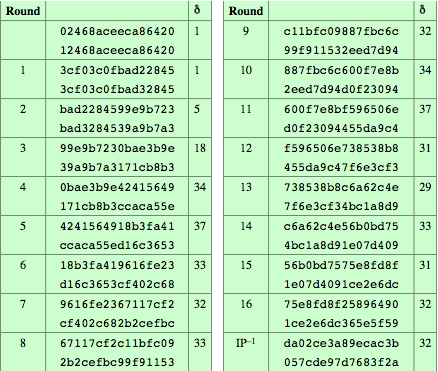
\includegraphics[width=0.85\textwidth]{../../images/python/page_033_img_01.png}

\end{document}
